\documentclass[journal,12pt,twocolumn]{IEEEtran}
\usepackage{setspace}
\usepackage{gensymb}
\usepackage{caption}
%\usepackage{multirow}
%\usepackage{multicolumn}
%\usepackage{subcaption}
%\doublespacing
\singlespacing
\usepackage{csvsimple}
\usepackage{amsmath}
\usepackage{multicol}
%\usepackage{enumerate}
\usepackage{amssymb}
%\usepackage{graphicx}
\usepackage{newfloat}
%\usepackage{syntax}
\usepackage{listings}
\usepackage{iithtlc}
\usepackage{color}
\usepackage{tikz}
\usetikzlibrary{shapes,arrows}



%\usepackage{graphicx}
%\usepackage{amssymb}
%\usepackage{relsize}
%\usepackage[cmex10]{amsmath}
%\usepackage{mathtools}
%\usepackage{amsthm}
%\interdisplaylinepenalty=2500
%\savesymbol{iint}
%\usepackage{txfonts}
%\restoresymbol{TXF}{iint}
%\usepackage{wasysym}
\usepackage{amsthm}
\usepackage{mathrsfs}
\usepackage{txfonts}
\usepackage{stfloats}
\usepackage{cite}
\usepackage{cases}
\usepackage{mathtools}
\usepackage{caption}
\usepackage{enumerate}	
\usepackage{enumitem}
\usepackage{amsmath}
%\usepackage{xtab}
\usepackage{longtable}
\usepackage{multirow}
%\usepackage{algorithm}
%\usepackage{algpseudocode}
\usepackage{enumitem}
\usepackage{mathtools}
\usepackage{hyperref}
%\usepackage[framemethod=tikz]{mdframed}
\usepackage{listings}
    %\usepackage[latin1]{inputenc}                                 %%
    \usepackage{color}                                            %%
    \usepackage{array}                                            %%
    \usepackage{longtable}                                        %%
    \usepackage{calc}                                             %%
    \usepackage{multirow}                                         %%
    \usepackage{hhline}                                           %%
    \usepackage{ifthen}                                           %%
  %optionally (for landscape tables embedded in another document): %%
    \usepackage{lscape}     


\usepackage{url}
\def\UrlBreaks{\do\/\do-}


%\usepackage{stmaryrd}


%\usepackage{wasysym}
%\newcounter{MYtempeqncnt}
\DeclareMathOperator*{\Res}{Res}
%\renewcommand{\baselinestretch}{2}
\renewcommand\thesection{\arabic{section}}
\renewcommand\thesubsection{\thesection.\arabic{subsection}}
\renewcommand\thesubsubsection{\thesubsection.\arabic{subsubsection}}

\renewcommand\thesectiondis{\arabic{section}}
\renewcommand\thesubsectiondis{\thesectiondis.\arabic{subsection}}
\renewcommand\thesubsubsectiondis{\thesubsectiondis.\arabic{subsubsection}}

% correct bad hyphenation here
\hyphenation{op-tical net-works semi-conduc-tor}

%\lstset{
%language=C,
%frame=single, 
%breaklines=true
%}

%\lstset{
	%%basicstyle=\small\ttfamily\bfseries,
	%%numberstyle=\small\ttfamily,
	%language=Octave,
	%backgroundcolor=\color{white},
	%%frame=single,
	%%keywordstyle=\bfseries,
	%%breaklines=true,
	%%showstringspaces=false,
	%%xleftmargin=-10mm,
	%%aboveskip=-1mm,
	%%belowskip=0mm
%}

%\surroundwithmdframed[width=\columnwidth]{lstlisting}
\def\inputGnumericTable{}                                 %%
\lstset{
%language=C,
frame=single, 
breaklines=true,
columns=fullflexible
}
 

\begin{document}
%
\tikzstyle{block} = [rectangle, draw,
    text width=3em, text centered, minimum height=3em]
\tikzstyle{sum} = [draw, circle, node distance=3cm]
\tikzstyle{input} = [coordinate]
\tikzstyle{output} = [coordinate]
\tikzstyle{pinstyle} = [pin edge={to-,thin,black}]

\theoremstyle{definition}
\newtheorem{theorem}{Theorem}[section]
\newtheorem{problem}{Problem}
\newtheorem{proposition}{Proposition}[section]
\newtheorem{lemma}{Lemma}[section]
\newtheorem{corollary}[theorem]{Corollary}
\newtheorem{example}{Example}[section]
\newtheorem{definition}{Definition}[section]
%\newtheorem{algorithm}{Algorithm}[section]
%\newtheorem{cor}{Corollary}
\newcommand{\BEQA}{\begin{eqnarray}}
\newcommand{\EEQA}{\end{eqnarray}}
\newcommand{\define}{\stackrel{\triangle}{=}}

\bibliographystyle{IEEEtran}
%\bibliographystyle{ieeetr}

\providecommand{\nCr}[2]{\,^{#1}C_{#2}} % nCr
\providecommand{\nPr}[2]{\,^{#1}P_{#2}} % nPr
\providecommand{\mbf}{\mathbf}
\providecommand{\pr}[1]{\ensuremath{\Pr\left(#1\right)}}
\providecommand{\qfunc}[1]{\ensuremath{Q\left(#1\right)}}
\providecommand{\sbrak}[1]{\ensuremath{{}\left[#1\right]}}
\providecommand{\lsbrak}[1]{\ensuremath{{}\left[#1\right.}}
\providecommand{\rsbrak}[1]{\ensuremath{{}\left.#1\right]}}
\providecommand{\brak}[1]{\ensuremath{\left(#1\right)}}
\providecommand{\lbrak}[1]{\ensuremath{\left(#1\right.}}
\providecommand{\rbrak}[1]{\ensuremath{\left.#1\right)}}
\providecommand{\cbrak}[1]{\ensuremath{\left\{#1\right\}}}
\providecommand{\lcbrak}[1]{\ensuremath{\left\{#1\right.}}
\providecommand{\rcbrak}[1]{\ensuremath{\left.#1\right\}}}
\theoremstyle{remark}
\newtheorem{rem}{Remark}
\newcommand{\sgn}{\mathop{\mathrm{sgn}}}
\providecommand{\abs}[1]{\left\vert#1\right\vert}
\providecommand{\res}[1]{\Res\displaylimits_{#1}} 
\providecommand{\norm}[1]{\lVert#1\rVert}
\providecommand{\mtx}[1]{\mathbf{#1}}
\providecommand{\mean}[1]{E\left[ #1 \right]}
\providecommand{\fourier}{\overset{\mathcal{F}}{ \rightleftharpoons}}
%\providecommand{\hilbert}{\overset{\mathcal{H}}{ \rightleftharpoons}}
\providecommand{\system}{\overset{\mathcal{H}}{ \longleftrightarrow}}
	%\newcommand{\solution}[2]{\textbf{Solution:}{#1}}
\newcommand{\solution}{\noindent \textbf{Solution: }}
\newcommand{\myvec}[1]{\ensuremath{\begin{pmatrix}#1\end{pmatrix}}}
\providecommand{\dec}[2]{\ensuremath{\overset{#1}{\underset{#2}{\gtrless}}}}
\DeclarePairedDelimiter{\ceil}{\lceil}{\rceil}
%\numberwithin{equation}{subsection}
%\numberwithin{equation}{section}
%\numberwithin{problem}{subsection}
%\numberwithin{definition}{subsection}
\makeatletter
\@addtoreset{figure}{section}
\makeatother

\let\StandardTheFigure\thefigure
%\renewcommand{\thefigure}{\theproblem.\arabic{figure}}
\renewcommand{\thefigure}{\thesection}


%\numberwithin{figure}{subsection}

%\numberwithin{equation}{subsection}
%\numberwithin{equation}{section}
%\numberwithin{equation}{problem}
%\numberwithin{problem}{subsection}
\numberwithin{problem}{section}
%%\numberwithin{definition}{subsection}
%\makeatletter
%\@addtoreset{figure}{problem}
%\makeatother
\makeatletter
\@addtoreset{table}{section}
\makeatother

\let\StandardTheFigure\thefigure
\let\StandardTheTable\thetable
\let\vec\mathbf
%%\renewcommand{\thefigure}{\theproblem.\arabic{figure}}
%\renewcommand{\thefigure}{\theproblem}

%%\numberwithin{figure}{section}

%%\numberwithin{figure}{subsection}



\def\putbox#1#2#3{\makebox[0in][l]{\makebox[#1][l]{}\raisebox{\baselineskip}[0in][0in]{\raisebox{#2}[0in][0in]{#3}}}}
     \def\rightbox#1{\makebox[0in][r]{#1}}
     \def\centbox#1{\makebox[0in]{#1}}
     \def\topbox#1{\raisebox{-\baselineskip}[0in][0in]{#1}}
     \def\midbox#1{\raisebox{-0.5\baselineskip}[0in][0in]{#1}}

\vspace{3cm}

\title{ 
	\logo{
Geometric Constructions through Python
	}
}

\author{ G V V Sharma$^{*}$% <-this % stops a space
	\thanks{*The author is with the Department
		of Electrical Engineering, Indian Institute of Technology, Hyderabad
		502285 India e-mail:  gadepall@iith.ac.in. All solutions in this manual is released under GNU 
GPL.  Free and open source.}
	
}	

\maketitle

\tableofcontents

\bigskip

\renewcommand{\thefigure}{\theenumi}
\renewcommand{\thetable}{\theenumi}

\begin{abstract}
This manual shows how to construct geometric figures using Python. The problems are based on  NCERT math 
textbooks of 
Class 9 and 10.
\end{abstract}
\section{Triangle}
\begin{enumerate}[label=\thesection.\arabic*
,ref=\thesection.\theenumi]
%
%\item Draw the rectangle $ABCD$ where $AB = c=6, BC = a= 8$.
%\\
\item Draw $\triangle ABC$  right angled at $\vec{B}$ such that $AB = 6, BC =8$.
\solution The coordinates are
\begin{align}
\label{eq:rt_tang_pair}
\vec{A}=\myvec{0 \\ c}
,
\vec{B}=\myvec{0 \\ 0}
,
\vec{C}=\myvec{0 \\ a}
\end{align}
\item Let $\vec{D}, \vec{F}, \vec{F}$ be the mid points of $BC,CA$ and $AB$ respectively in $\triangle ABC$. Draw $AD,BE$ and $CF$.
\\
\solution 
\begin{align}
\label{eq:rt_tang_pair}
\vec{D} = \frac{\vec{B}+\vec{C}}{2}
\\
\vec{E} = \frac{\vec{C}+\vec{A}}{2}
\\
\vec{F} = \frac{\vec{A}+\vec{B}}{2}
\end{align}
\item  Draw $AD, BE$ and $CF$.
\item Draw $\triangle DEF$ in the previous problem.

\end{enumerate}
\section{Circle}
\begin{enumerate}[label=\thesection.\arabic*
,ref=\thesection.\theenumi]
\item Now redraw $\triangle ABC$ with 
\begin{align}
\label{eq:rt_triang_circum}
\vec{O}=\frac{\vec{A}+\vec{C}}{2}=\myvec{0 \\0}
\end{align}
\item Draw the circumcircle of  $\triangle ABC$ with centre $\vec{O}$.  
\\
\solution The radius of the circumcircle is 
\begin{align}
\label{eq:rt_triang_circum_rad}
r=\frac{b}{2}=\frac{\sqrt{a^2+c^2}}{2}
\end{align}
%\item Now redraw $\triangle ABC$ with 
%\begin{align}
%\vec{A}=\myvec{0 \\0}
%\end{align}
%\\
%\solution The new coordinates are
%\begin{align}
%\vec{B}=\myvec{0 \\-c}
%\vec{C}=\myvec{0 \\a-c}
%\end{align}
\item Draw a circle with centre 
\begin{align}
\vec{A}=\myvec{0 \\0}
\end{align}
%
$\vec{A}$ 
and radius $c$.
\item For 
\begin{align}
\vec{C}=\myvec{b \\0}, 
\end{align}
find $p,q$ such that
\begin{align}
\vec{B}=\myvec{p \\q}, 
\end{align}
\item Redraw $\triangle ABC$ with centre $\vec{A}$ and radius $c$.
\item Draw the tangent $CD$ to the circle.
\\
\solution The coordinate
\begin{align}
\label{eq:rt_tang_pair}
D=\myvec{p \\ -q}
\end{align}
The following code draws the circle and tangents in Fig. \ref{fig:circle}
\lstinputlisting{./codes/draw_circle.py}
%
\begin{figure}
\centering
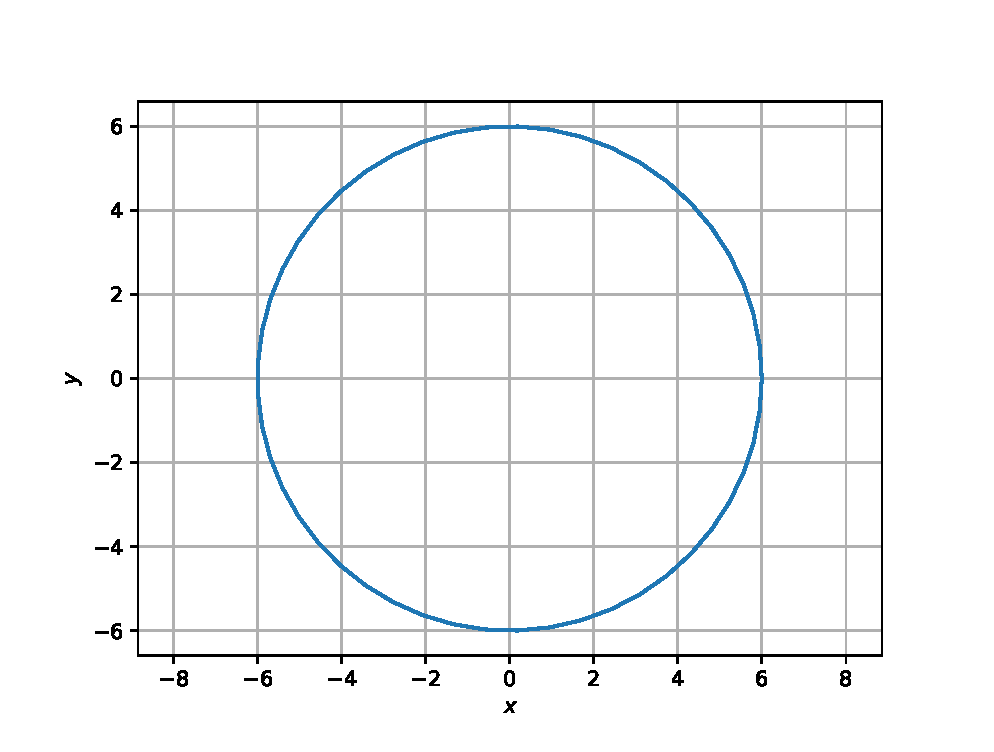
\includegraphics[width=\columnwidth]{./figs/circle.eps}
\caption{}
\label{fig:circle}
\end{figure}
%
\item Consider $\triangle ABC$ with $BC = a, CA = b$ and $AB= c$.  Let
\begin{align}
\label{eq:triangle_coord_def}
\vec{A}=\myvec{p \\q},
\vec{B}=\myvec{0 \\0},
\vec{C}=\myvec{0 \\a}
\end{align}
Find  $p$ and $q$.
\\
\solution 
%
Since
\begin{align}
\label{eq:triangle_dist}
p^2+q^2&= c^2
\\
\brak{p-a}^2+q^2&= b^2,
\end{align}
we obtain
\begin{align}
p = \frac{a^2+c^2-b^2}{2a},
q = \sqrt{c^2-p^2}
\end{align}
%
\item Plot $\triangle ABC$ for $a = 8, b = 11$ and $c = 13$. 
\\
\solution The following program plots $\triangle ABC$ in Fig. \ref{fig:triangle}
\lstinputlisting{./codes/draw_triangle.py}
%
\begin{figure}
\centering
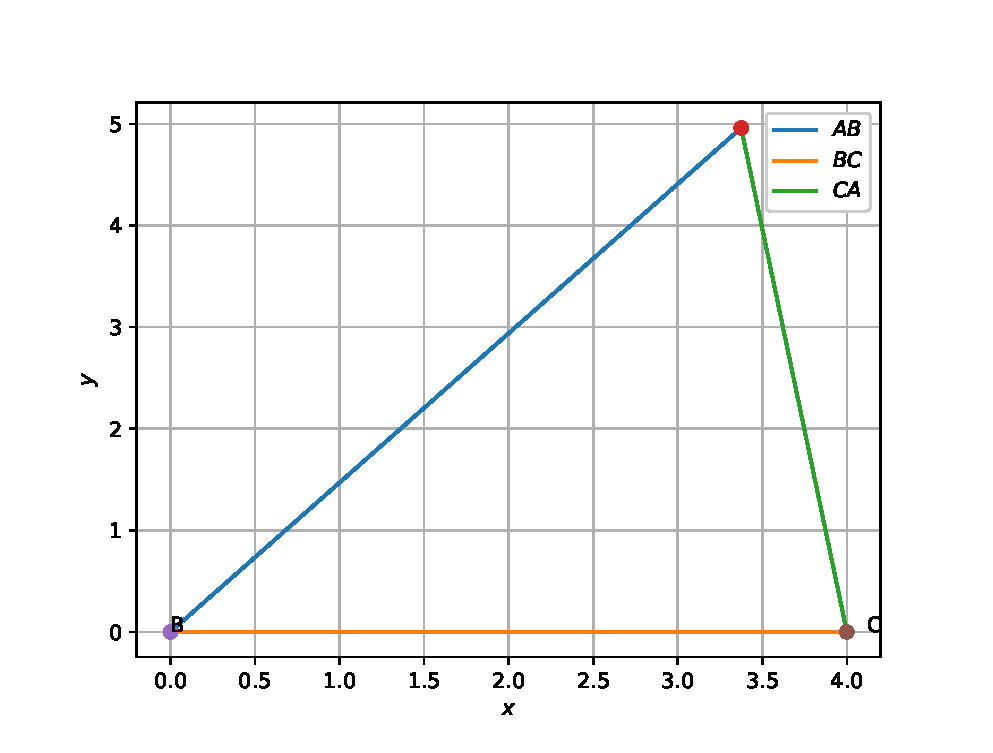
\includegraphics[width=\columnwidth]{./figs/triangle.eps}
\caption{}
\label{fig:triangle}
\end{figure}
\item Find $\vec{O}$ and $R$ such that 
\begin{align}
R = OA = OB = OC
\end{align}
\item Let
\begin{align}
\label{eq:tang_len}
x+y = a
y+z = b
z+x = c
\end{align}
Find $x,y,z$.
\\
\solution  The given information can be expressed as the matrix equation
\begin{align}
\myvec{
1 & 1 & 0
\\
0 & 1 & 1
\\
1 & 0 & 1
}
\myvec{x \\ y \\ z} = \myvec{a \\b\\c}
\end{align}
%
which can be solved to obtain $x,y,z$.
\item Find $\vec{D}, \vec{E}, \vec{F}$ such that 
\begin{align}
\label{eq:incircle}
AE = AF = z
BE = BD = x
CD = CF = y
\end{align}
\item Find $\vec{I}$ such that 
\begin{align}
\label{eq:inradius}
ID = IE = IF =r
\end{align}

\end{enumerate}
%
\section{Exercises}
\begin{enumerate}[label=\thesection.\arabic*
,ref=\thesection.\theenumi]
\item Draw a circle with centre $\vec{B}$ and radius 6.  If $\vec{C}$ be  a point 10 units  away from its 
centre, construct the pair of tangents $AC$ and $CD$ to the 
circle.
\\
\solution From the given information, in $\triangle ABC, AC \perp AB, a = 
10$ and $c = 6$.
\begin{align}
b =  \sqrt{a^2-c^2}
\end{align}
\item Write a program to compute $p$ and $q$ when $a = 8, b = 11$ and $c = 13$. 
\item In $\triangle ABC$,  $a$ and  $\angle B$ are known and $b+c = k$. If 
\begin{align}
\label{eq:cos_formula}
b^2  = a^2+c^2- 2ac \cos B
\end{align}
%
find $b$ and $c$.
\\
\solution From \eqref{eq:cos_formula}, 
\begin{align}
\label{eq:aB}
\brak{k-c}^2 &= a^2+c^2- 2ac \cos B
\\
\implies k^2 -2kc+c^2 &= a^2+c^2- 2ac \cos B
\\
\implies -2kc+ 2ac \cos B&= a^2-k^2 
\\
\implies 2c\brak{a \cos B -k}&= a^2-k^2 
\\
\text{or, } c &= \frac{ a^2-k^2 }{2\brak{a \cos B -k}}
\end{align}

\item In $\triangle ABC$,  $a = 7, \angle B = 75^{\degree}$ and $b+c = 13$. 
%If 
%\begin{align}
%\label{eq:cos_formula}
%a^2+c^2-b^2 = 2ac \cos B
%\end{align}
Find $b$ and $c$ and sketch $\triangle ABC$.
\item In $\triangle ABC$,  $a = 8, \angle B = 45^{\degree}$ and $c-b = 3.5$.
Sketch $\triangle ABC$.
\item In $\triangle ABC$,  $a = 6, \angle B = 60^{\degree}$ and $b-c = 2$. 
Sketch $\triangle ABC$.
\item $\triangle ABC$ is right angled at $\vec{B}$.  If $a = 12$ and $b+c = 18$, find $a,b,c$ and draw the 
triangle.
\\
\solution From Baudhayana's theorem, 
\begin{align}
b^2 = a^2 + c^2
\end{align}
%Hence, 
%\begin{align}
%\brak{18-c}^2 &= a^2 + c^2
%\implies c &= \frac{18^2-a^2}{36} = 5
%\end{align}
%%
%and $b = 13$.
%
\item In $\triangle ABC$,  given that $a+b+c = 11, \angle B = 45^{\degree}$ and $\angle C = 45^{\degree}$, 
find 
$a,b,c$.
\\
\solution We have
\begin{align}
a = b \cos C + c \cos B
\\
b \sin C = c \sin B
\\
a + b+c = 11
\end{align}
%
resulting  in the matrix equation 
\begin{align}
\begin{pmatrix}
1 & -\cos C & - \cos B
\\
0 & \sin C &- \sin B
\\
1 & 1 & 1
\end{pmatrix}
%\myvec{
%}
\myvec{a \\b\\c} = \myvec{0 \\ 0 \\ 11}
\end{align}

Solving the equivalent matrix equation gives the desired answer.
\item Draw $\triangle ABC$,  given that $a+b+c = 11, \angle B = 30^{\degree}$ and $\angle C = 90^{\degree}$, 
find 
$a,b,c$.
\item Draw a square of side $3$.
\item Draw a parallelogram with sides $12$ and $5$.

\item Draw a circle with centre $\vec{O}$ and diameter $AC = 6$.  Choose any point $B$ on the circle and draw $\triangle ABC$.
\item In $\triangle ABC$, $a =8, b = 11, c = 13$. Find 
\begin{align}
R = \frac{a}{2\sin A}.
\end{align}
%
Let $\vec{D}$ be the mid point of $BC$.  Find the point $\vec{O}$ such that $\triangle ODB$ is right angled at $\vec{D}$ and $OD=R$. Draw the circle with centre $\vec{O}$ and radius $R$.
\item Let 
\begin{align}
r = \frac{abc}{2\brak{a+b+c}}.
\end{align}
and 
\begin{align}
IB = r\sqrt{\frac{2}{1-\cos B}}.
\end{align}
%
Draw a circle with centre $\vec{I}$ and radius $r$.

\item Construct a tangent to a circle of radius 4 units from a point on the concentric circle of radius 6 
units.
\item Draw a circle of radius 3 units. Take  two points $\vec{P}$ and $\vec{Q}$ on one of its extended 
diameter each at a distance of 7 units from its centre. Draw tangents to the circle from these two points 
$\vec{P}$ and $\vec{Q}$.
\item Draw a pair of tangents to a circle of radius 5 units which are inclined to each other at an angle of 
$60^{\degree}$.
\item Draw a line segment $AB$ of length 8 units. Taking $\vec{A}$ as centre, draw a circle of radius 4 units 
and taking $\vec{B}$ as centre, draw another circle of radius 3 units. Construct tangents to each circle from 
the centre of the other circle.
\item Let ABC be a right triangle in which $a = 8, c = 6$ and $\angle B = 90^{\degree}$.  $BD$ is the 
perpendicular from $\vec{B}$ on $AC$. The circle through $\vec{B}, \vec{C}, \vec{D}$ is drawn.  Construct the 
tangents from $\vec{A}$ to this circle.
\end{enumerate}
\end{document}


